% =============================================================================
% KAPITEL 6 – Konzeption der Observability-Strategie (GEKÜRZT)
% =============================================================================
 
 
\chapter{Konzeption der Observability-Strategie für frag.jetzt}
 
Die vorangegangenen Kapitel haben den theoretischen Bezugsrahmen gelegt, den Ist-Zustand von frag.jetzt analysiert und den Observability-Stack begründet ausgewählt. Das vorliegende Kapitel überführt diese Vorarbeiten in eine zusammenhängende Strategie und beantwortet, \emph{was} beobachtet werden soll, \emph{warum} gerade diese Größen betrieblich bedeutsam sind und \emph{nach welchen Prinzipien} die Lösung aufgebaut wird.
 
 
\section{Leitprinzipien der Strategie}
\label{sec:leitprinzipien}
 
Vier Prinzipien greifen die Anforderungen A1--A5 aus Kapitel~3 auf und übersetzen sie in Gestaltungsleitlinien für die nachfolgenden Entwurfsentscheidungen.
 
\paragraph{P1: Servicebezogene Messbarkeit.}
Jeder Dienst von frag.jetzt wird als eigenständige Beobachtungseinheit behandelt, für die Messgrößen entlang der vier Golden Signals abgeleitet werden. Das Vorgehen folgt der Empfehlung, Beobachtungsgrößen an den Schnittstellen der Dienste zu erheben, weil sich dort Symptome manifestieren, bevor tieferliegende Ursachen sichtbar werden \parencite[S.~59]{ewaschukMonitoringDistributedSystems}. Anforderung~A2 wird damit unmittelbar adressiert.
 
\paragraph{P2: Ende-zu-Ende-Nachvollziehbarkeit.}
An jedem der in Abschnitt~3.2 identifizierten Dienstübergänge muss Trace-Kontext propagiert werden, damit kausal zusammenhängende Aktivitäten über Dienstgrenzen hinweg korrelierbar bleiben \parencite[S.~32]{bissig2024unified}. Ohne diese Verknüpfung bleiben Logs und Metriken isolierte Datenpunkte \parencite[S.~14--15]{sundstrom2025finding}. Das Prinzip greift Anforderung~A1 und den Korrelationsaspekt von A3 auf.
 
\paragraph{P3: Rollenorientierte Aufbereitung.}
Unterschiedliche Stakeholder stellen unterschiedliche Fragen an dasselbe Laufzeitverhalten \parencite[S.~54]{bissig2024unified}. Abschnitt~6.5 überführt dieses Prinzip in drei konkrete Sichtebenen.
 
\paragraph{P4: Schrittweise Erweiterbarkeit.}
Da frag.jetzt Observability erstmals einführt und knappe Ressourcen eine eigenständige Herausforderung darstellen \parencite[S.~9--10]{Niedermaier2019onObservability}, wird die Strategie als erweiterbarer Ausgangspunkt angelegt. Die Instrumentierung über OpenTelemetry stellt sicher, dass Backend-Komponenten austauschbar bleiben \parencite[S.~502]{gudimetla2025transitioning}.
 
 
\section{Logische Zielarchitektur der Observability}
\label{sec:zielarchitektur}
 
Die Observability-Architektur folgt einem vierstufigen Schichtenmodell, wie es \textcite[S.~73037--73038]{kosinska2023toward} als grundlegendes Muster für cloud-native Anwendungen beschreiben. Abbildung~\ref{fig:zielarchitektur-observability} zeigt den Datenfluss von der Instrumentierung über Sammlung und Speicherung bis zur Auswertung. Die werkzeugspezifische Konfiguration wird in Kapitel~7 dokumentiert.
 
\begin{figure}[htb]
\centering
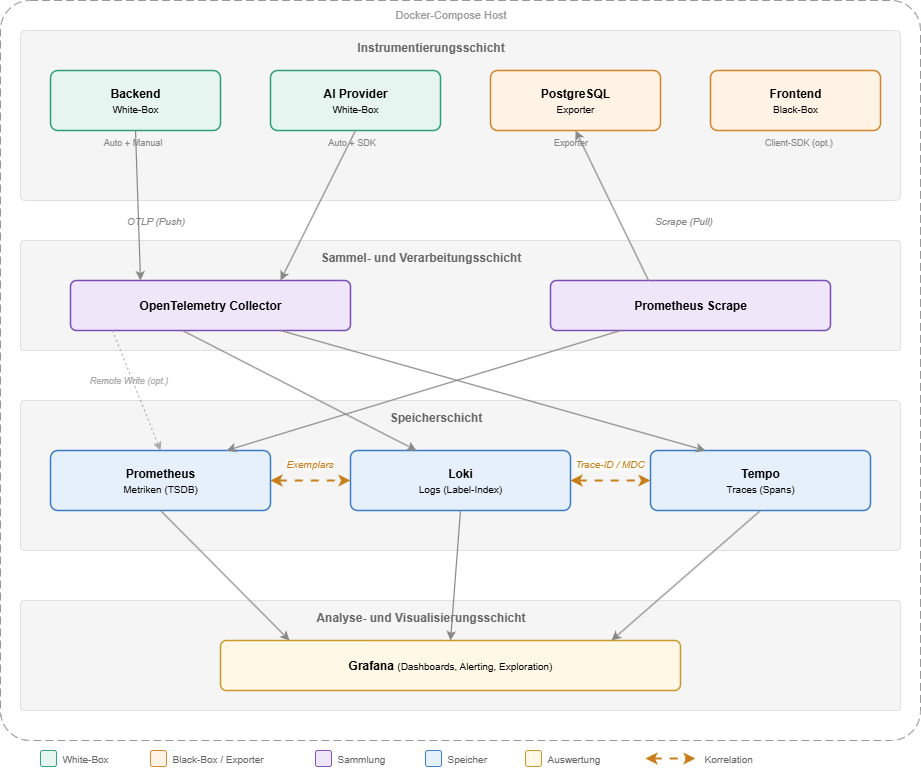
\includegraphics[width=0.95\textwidth]{images/fig_zielarchitektur.png}
\caption[Logische Zielarchitektur der Observability-Pipeline fuer frag.jetzt]{Logische Zielarchitektur der Observability-Pipeline fuer frag.jetzt. Gestrichelte Querverbindungen kennzeichnen Korrelationsmechanismen zwischen den Speicher-Backends. \small Quelle: Eigene Darstellung.}
\label{fig:zielarchitektur-observability}
\end{figure}


\subsection{Instrumentierungsschicht}
 
Aus der Architektur von frag.jetzt ergibt sich eine differenzierte Instrumentierungsstrategie. Backend, WebSocket Gateway und AI Provider sind als Eigenentwicklungen über Auto-Instrumentierung mit selektiver manueller Ergänzung beobachtbar. Die Quellcodeanalyse in Kapitel~3 hat gezeigt, dass keine dieser Komponenten bislang Telemetrie emittiert (R3). Demgegenüber agieren die externen LLM-Provider als Black-Box-Abhängigkeiten, bei denen mindestens die Ein- und Ausgangsseite jedes Aufrufs instrumentiert werden muss \parencite[S.~31]{bissig2024unified}.
 
OpenTelemetry übernimmt die Rolle der standardisierten Instrumentierungsschicht (vgl.~Abschnitt~5.2). Die entscheidenden Übergabepunkte für die Kontextpropagation sind die Verbindungen zwischen Frontend und Reverse-Proxy, zwischen Reverse-Proxy und Backend, zwischen Backend und Datenbank sowie zwischen Backend und AI Provider. Eine besondere Herausforderung stellt die Echtzeitkommunikation über den Message Broker dar, da dort eine manuelle Injektion des Trace-Kontexts in das Nachrichtenformat erforderlich wird \parencite[S.~25]{sundstrom2025finding}. Ergänzend werden Container-Metriken und datenbankspezifische Indikatoren über spezialisierte Exporter erhoben, die Prometheus-kompatible Endpunkte bereitstellen.
 
 
\subsection{Sammel- und Verarbeitungsschicht}
 
Der OpenTelemetry Collector fungiert als zentrale Routing-Komponente, die Instrumentierung und Backend entkoppelt \parencite[S.~107]{sakinala2025observability}; \parencite[S.~502]{gudimetla2025transitioning}. Für frag.jetzt wird der Collector als pushbasierte Empfangskomponente für anwendungsseitige Traces und Metriken konfiguriert, weil ein Push-Modell bei einer zukünftigen Erweiterung keine Umstellung erfordert \parencite[S.~39]{bissig2024unified}. Infrastrukturmetriken folgen dagegen dem etablierten Pull-Modell über Prometheus-Scraping. Bei dem für frag.jetzt erwarteten geringen Datenvolumen kann zunächst auf Sampling verzichtet werden. Eine Anpassung ist erst dann vorgesehen, wenn das Telemetrievolumen die Speicherkapazität des Hosts belastet.
 
 
\subsection{Speicherschicht}
 
Die aufbereiteten Signale werden in drei spezialisierten Backends abgelegt: Metriken in der lokalen Prometheus-TSDB, Logs in Loki mit labelbasierter Indexierung und Traces in Tempo. Entscheidend ist die Korrelierbarkeit über die drei Speicher hinweg, die bei getrennter Speicherung nicht automatisch entsteht \parencite[S.~44]{bissig2024unified}. Drei Mechanismen bilden die diagnostischen Brücken: die Trace-ID als gemeinsamer Identifikator über alle drei Pfeiler, die Injektion der Trace-ID in den Mapped Diagnostic Context (MDC) des Logging-Frameworks \parencite[S.~20]{sundstrom2025finding} und Metriken-Exemplars, die den direkten Übergang von einem aggregierten Metrikwert zum zugehörigen Trace ermöglichen \parencite[S.~25]{bissig2024unified}; \parencite[S.~12]{albuquerque2025tracing}. Die Speichertrennung ist nur dann diagnostisch tragfähig, wenn diese Verknüpfungspfade von Beginn an in der Instrumentierung verankert werden.
 
 
\subsection{Analyse- und Visualisierungsschicht}
 
Grafana bildet die einheitliche Oberfläche für Abfrage, Visualisierung und Alarmierung aller gespeicherten Telemetriedaten \parencite[S.~16]{sundstrom2025finding}. Die Korrelation wird über Datenquellen-übergreifende Navigation hergestellt: Von einem auffälligen Metrikpunkt lässt sich über ein Exemplar direkt zum zugehörigen Trace springen, und aus einem Trace heraus führen verknüpfte Logabfragen zum relevanten Kontext.
 
 
\subsection{Einordnung im Kontext von frag.jetzt}
 
Die beschriebene Vier-Schichten-Architektur orientiert sich an Referenzmodellen für Kubernetes-basierte Umgebungen \parencite[S.~501]{gudimetla2025transitioning}. frag.jetzt weicht davon in drei Punkten ab. Erstens läuft das Ökosystem auf einem einzelnen Host, sodass der Collector nicht als Sidecar, sondern als eigenständiger Container betrieben wird. Zweitens fehlt ein Service Mesh, weshalb die Telemetrieerzeugung vollständig auf Anwendungsebene erfolgen muss. Drittens erlaubt das geringe Telemetrievolumen einen Verzicht auf Sampling und vorgelagerte Aggregation, erfordert aber eine bewusste Kapazitätsbeobachtung bei wachsendem Einsatz. Die Architektur hält den Einstieg bewusst schlank und lässt Erweiterungspfade wie Mimir für Langzeitmetriken oder Tail-Based Sampling offen, ohne die Grundstruktur zu verändern \parencite[S.~1--2]{borges2024informed}.
 
 
\section{Servicebezogene Operationalisierung der Four Golden Signals}
\label{sec:golden-signals-operationalisierung}
 
Die Ableitung der Beobachtungsgrößen folgt dem in Abschnitt~4.2 beschriebenen Vorgehen und konzentriert sich auf die vier für die Forschungsfragen zentralen Beobachtungseinheiten: Frontend, Backend, Datenbank und externe KI-Dienste. Nginx, RabbitMQ und das WebSocket Gateway werden als Infrastruktur- bzw.\ Integrationskomponenten über die Infrastrukturmetriken mitbeobachtet, erhalten aber keine eigenständige Signal-Matrix. \textcite[S.~60]{ewaschukMonitoringDistributedSystems} bezeichnet die Wahl des Traffic-Indikators ausdrücklich als \emph{high-level system-specific metric}, was bedeutet, dass die Übertragung der vier Dimensionen auf jeden Dienst eine eigenständige Entwurfsleistung erfordert. Tabelle~\ref{tab:signal-matrix} fasst die Ergebnisse dieser Ableitung in einer Signal-Matrix zusammen. Die folgenden Unterabschnitte erläutern nur die Besonderheiten, die sich nicht unmittelbar aus der Matrix erschließen.
 
 
\subsection{PWA-Frontend}
\label{sec:gs-frontend}
 
Das Angular-Frontend unterscheidet sich grundlegend von den serverseitigen Komponenten, weil die Ausführung im Browser stattfindet und die Infrastruktur nicht direkt kontrollierbar ist. Aus Nutzersicht manifestiert sich Latenz als wahrgenommene Ladezeit, zu der neben der Server-Antwortzeit auch clientseitige Faktoren wie Netzwerkqualität und Rendering beitragen. Basisindikatoren sind die Dauer von API-Aufrufen und die Ende-zu-Ende-Ladezeit beim Betreten eines Raums. Browserbasierte Metriken wie First Contentful Paint über das OpenTelemetry-Browser-SDK sind als optionale Erweiterung zu verstehen.
 
Die Nachfrageintensität lässt sich über aktive WebSocket-Verbindungen und HTTP-Anfragen pro Zeiteinheit messen. Fehlerindikatoren umfassen fehlgeschlagene API-Aufrufe (4xx/5xx), unbehandelte JavaScript-Exceptions und WebSocket-Verbindungsabbrüche. Klassische Sättigungsmetriken wie CPU und Speicher beziehen sich auf das Endgerät und liegen außerhalb des Einflussbereichs des Betriebsteams. Da die Grenzen der Frontend-Beobachtbarkeit eng gesteckt sind, liegt der instrumentierungstechnische Schwerpunkt auf den serverseitigen Komponenten.
 
 
\subsection{Spring-Boot-Backend}
\label{sec:gs-backend}
 
Das Backend ist die zentrale Verarbeitungskomponente und der in Kapitel~3 identifizierte kritische Punkt. Der primäre Latenzindikator ist die Antwortdauer je REST-Endpunkt als Histogramm (p50, p95, p99), weil Durchschnittswerte die Erfahrung langsam bedienter Nutzer verbergen können \parencite[S.~60]{ewaschukMonitoringDistributedSystems}. Ebenso muss die Latenz erfolgreicher und fehlgeschlagener Anfragen getrennt erfasst werden, da schnell zurückgegebene Fehler den Gesamtdurchschnitt verzerren. Ergänzend werden die Latenzen ausgehender Aufrufe an PostgreSQL, den Message Broker und den AI Provider separat erhoben. Das reaktive Programmiermodell auf Basis von WebFlux erfordert dabei besondere Aufmerksamkeit, da die Messung auf Span-Ebene innerhalb der reaktiven Kette erfolgen muss \parencite[S.~25]{sundstrom2025finding}.
 
Die Anfragerate pro Endpunkt bildet den Traffic ab. Für die geschäftskritischen Abläufe aus Abschnitt~3.3 ist eine gesonderte Erfassung sinnvoll. Fehler werden auf mehreren Ebenen erfasst: HTTP-5xx-Statuscodes, unbehandelte Exceptions und fehlgeschlagene Downstream-Aufrufe. Da kein externer Aufruf einen Timeout besitzt (R1), äußern sich Timeout-bedingte Fehler als hängende Anfragen, was die Latenzüberwachung umso dringlicher macht. Die Sättigung wird über Container-Metriken und den R2DBC-Connection-Pool gemessen. \textcite[S.~60--61]{ewaschukMonitoringDistributedSystems} empfiehlt, Sättigung indirekt über steigende Latenz am 99.\,Perzentil zu erkennen, weil Latenzzunahmen häufig ein Frühindikator für Ressourcenerschöpfung sind.
 
 
\subsection{PostgreSQL}
\label{sec:gs-postgresql}
 
Die Datenbank ist an allen drei geschäftskritischen Nutzungspfaden beteiligt. Die Vote-Trigger und die Comment-Nummern-Generierung (Abschnitt~3.3) erzeugen potenzielle Engpässe. Der zentrale Latenzindikator ist die Abfrageausführungszeit, wobei lang laufende Abfragen auf fehlende Indizes oder Row-Level Contention hindeuten. Die Transaktionsrate und die aktive Verbindungszahl bilden den Traffic ab. Relevante Fehlersignale umfassen Deadlocks, fehlgeschlagene Transaktionen und Verbindungsablehnungen. Die Sättigung wird über das Verhältnis genutzter zu maximal verfügbarer Verbindungen, die Buffer-Cache-Hit-Rate und die Disk-I/O-Auslastung gemessen. Ein sinkender Cache-Hit-Anteil deutet darauf hin, dass die Arbeitsspeicherkonfiguration nicht mehr zum Datenvolumen passt.
 
 
\subsection{Externe KI-Dienste}
\label{sec:gs-ki}
 
Die Beobachtung der externen KI-Dienste beschränkt sich auf die Schnittstelle zwischen AI Provider und den angebundenen Modellen, da der Quellcode der LLM-Provider nicht verfügbar ist \parencite[S.~31]{bissig2024unified}. Die LLM-Antwortzeit wird als Histogramm pro Provider und Modell erfasst. Da kein Timeout konfiguriert ist (R1), kann ein einzelner hängender Aufruf den AI Provider blockieren und über die Aufrufkette das Backend beeinflussen. Der Traffic wird als Anzahl der LLM-Aufrufe pro Zeiteinheit je Funktionstyp gemessen. Fehlersignale sind HTTP-Fehlerantworten der Provider-APIs (insbesondere 429 Rate Limit Exceeded), Timeouts und Parsing-Fehler. Neun von 19~LLM-Providern sind explizit mit \texttt{max\_retries=0} konfiguriert, sodass ein fehlgeschlagener Aufruf unmittelbar durchschlägt. Da die LLM-Provider keinen Einblick in ihre Ressourcenauslastung gewähren, wird Sättigung über Proxy-Indikatoren wie steigende Antwortzeiten und zunehmende Rate-Limit-Fehler abgebildet.
 
 
\section{Serviceübergreifende Signal-Matrix}
\label{sec:signal-matrix}
 
Tabelle~\ref{tab:signal-matrix} verdichtet die vorangehenden Ableitungen in einer Gesamtübersicht. Sie bildet die Grundlage für das rollenbasierte Dashboard-Design (Abschnitt~6.5) und definiert den Rahmen für das Alerting-Konzept (Abschnitt~6.6), weil nicht jede Messgröße Alarmrelevant ist.
 
\begin{table}[htb]
\centering
\caption[Serviceübergreifende Signal-Matrix mit Zuordnung von Dienst, Golden Signal, Messgröße, Erhebungszweck und primärer Stakeholder-Rolle.]{Serviceübergreifende Signal-Matrix mit Zuordnung von Dienst, Golden Signal, Messgröße, Erhebungszweck und primärer Stakeholder-Rolle. \small Quelle: Eigene Darstellung.}
\label{tab:signal-matrix}
\small
\begin{tabularx}{\textwidth}{
  >{\RaggedRight\arraybackslash}p{1.6cm}
  >{\RaggedRight\arraybackslash}p{1.5cm}
  >{\RaggedRight\arraybackslash}p{5.9cm}
  >{\RaggedRight\arraybackslash}X
  >{\RaggedRight\arraybackslash}p{1.8cm}
}
\toprule
\textbf{Dienst} & \textbf{Signal} & \textbf{Messgröße} & \textbf{Zweck} & \textbf{Rolle} \\
\midrule
Backend   & Latency    & Antwortdauer je Endpunkt (p50, p95, p99)         & Nutzererfahrung, Engpasserkennung   & Entwicklung \\
Backend   & Traffic    & Anfragen/s je Pfad, Broker-Nachrichten/s          & Lastbild, Kapazitätsplanung         & DevOps \\
Backend   & Errors     & HTTP-5xx-Rate, Exception-Rate, Downstream-Fehler  & Fehlererkennung, Trendanalyse       & Entwicklung \\
Backend   & Saturation & CPU, Speicher, R2DBC-Pool-Nutzung                 & Ressourcenwarnung                   & DevOps \\[4pt]
PostgreSQL & Latency   & Abfrageausführungszeit (Durchschnitt, Maximum)     & Indexbedarf, Contention-Erkennung   & Entwicklung \\
PostgreSQL & Traffic   & Transaktionen/s, aktive Verbindungen               & Nutzungsintensität                  & DevOps \\
PostgreSQL & Errors    & Deadlocks, fehlgeschl.\ Transaktionen, Lock-Waits  & Stabilitätsüberwachung              & Entwicklung \\
PostgreSQL & Saturation & Verbindungspool-Quote, Cache-Hit-Rate, Disk-I/O   & Kapazitätswarnung                   & DevOps \\[4pt]
AI Prov.  & Latency    & LLM-Antwortzeit je Provider/Modell (Histogramm)    & SLA-Proxy, Kaskadenerkennung       & Entwicklung \\
AI Prov.  & Traffic    & LLM-Aufrufe/Zeiteinheit je Funktionstyp            & Nutzungsmuster, Kontingentplanung  & Product Owner \\
AI Prov.  & Errors     & Provider-Fehlerrate, 429er-Rate, Parsing-Fehler   & Verfügbarkeit ext.\ Abhängigkeiten & Entwicklung \\
AI Prov.  & Saturation & Antwortzeit-Trend, Rate-Limit-Häufigkeit, lokale CPU & Kapazitätswarnung               & DevOps \\[4pt]
Frontend  & Latency    & API-Aufruf-Dauer, Raum-Ladezeit                    & Nutzererfahrung                    & Product Owner \\
Frontend  & Traffic    & Aktive WS-Verbindungen, HTTP-Anfragen/s            & Nutzungsgrad                       & Product Owner \\
Frontend  & Errors     & HTTP-Fehler, JS-Exceptions, WS-Abbrüche           & Fehlererkennung clientseitig       & Entwicklung \\
Frontend  & Saturation & Antwortzeit-Trend, Retry-Häufigkeit                & Überlastindikation                 & DevOps \\
\bottomrule
\end{tabularx}
\end{table}
 
 
\section{Rollenbasiertes Informations- und Dashboard-Konzept}
\label{sec:dashboard-konzept}
 
Für frag.jetzt wird eine hierarchische Informationsarchitektur in drei Sichtebenen umgesetzt, deren Zuschnitt sich aus den Stakeholder-Gruppen und der Signal-Matrix ableitet \parencite[S.~108]{sakinala2025observability}.
 
\paragraph{Übersichtssicht (Product Owner / Management).}
Diese Ebene beantwortet die Frage, ob frag.jetzt aus Nutzersicht funktioniert. Sie zeigt verdichtete Indikatoren wie aktive Raumsitzungen, globale Fehlerrate und Gesamtlatenz der Kernabläufe. Detailinformationen sind nur über Verlinkung erreichbar.
 
\paragraph{Dienst- und Infrastruktursicht (DevOps / Betrieb).}
Diese Ebene beantwortet die Frage, wo das Problem liegt. Sie stellt Ressourcenmetriken je Container, Datenbankauslastung, Message-Broker-Kennzahlen und eine aus Trace-Daten gewonnene Service-Map dar.
 
\paragraph{Diagnose- und Entwicklungssicht (Entwicklung).}
Diese Ebene beantwortet die Frage, was genau im Code passiert. Sie bietet endpunktbezogene Latenzhistogramme, Fehleraufschlüsselungen, Trace-Ansichten und die Möglichkeit, aus einem Trace in die zugehörigen Logeinträge zu springen. Die technische Umsetzung wird in Kapitel~7 dokumentiert.
 
 
\section{Alerting-Konzept und Runbook-Logik}
\label{sec:alerting-konzept}
 
Aufbauend auf den in Abschnitt~2.7 erarbeiteten Grundlagen folgt das Alerting-Konzept drei Grundsätzen. Alarme reagieren symptomorientiert auf nutzerwirksame Zustände statt auf interne Ursachenindikatoren \parencite[S.~63--64]{ewaschukMonitoringDistributedSystems}. Jeder Alarm muss handlungsfähig sein, also Problem, betroffene Komponente und empfohlene Erstmaßnahme erkennbar machen \parencite[S.~174]{vinnakota2025creating}. Schweregrade orientieren sich an der Nutzerwirkung: \emph{Critical} für akute Ausfälle geschäftskritischer Funktionen, \emph{Warning} für sich abzeichnende Verschlechterungen.
 
 
\subsection{Alarmkategorien}
 
Aus der Signal-Matrix lassen sich vier Kategorien ableiten. Die konkreten Schwellenwerte und Zeitfenster werden in Kapitel~7 festgelegt.
 
\paragraph{Verfügbarkeitsalarme (Critical).}
Ein Alarm wird ausgelöst, wenn eine geschäftskritische Funktion nicht mehr erreichbar ist, etwa wenn das Backend über einen definierten Zeitraum keine erfolgreichen Antworten liefert oder die Datenbankverbindung dauerhaft fehlschlägt.
 
\paragraph{Latenzalarme (Warning / Critical).}
Steigt die Antwortzeit eines Kernendpunkts über einen definierten Grenzwert, etwa das 95.\,Perzentil über ein gleitendes Fenster, wird zunächst eine Warnung und bei weiterer Verschlechterung ein kritischer Alarm erzeugt. Für die KI-Dienste gelten angepasste Grenzwerte.
 
\paragraph{Fehleralarme (Warning / Critical).}
Eine Fehlerrate oberhalb eines definierten Anteils löst eine Warnung aus. Die explizite Trennung von client- (4xx) und serverseitigen (5xx) Fehlern verhindert, dass ungültige Eingaben denselben Alarm wie interne Serverfehler erzeugen.
 
\paragraph{Sättigungsalarme (Warning).}
Ressourcenmetriken wie CPU-Auslastung und Datenbankverbindungspool-Nutzung werden als vorausschauende Warnung konfiguriert. \textcite[S.~60--61]{ewaschukMonitoringDistributedSystems} empfiehlt, Sättigung indirekt über steigende Latenz am 99.\,Perzentil zu erkennen.
 
 
\subsection{Runbook-Verknüpfung}
 
Jeder Critical-Alarm wird mit einem Runbook verknüpft, das Problembeschreibung, betroffene Komponente, Diagnoseschritte, Erstmaßnahmen und Eskalationspfad enthält. Für den Prototyp werden exemplarische Runbooks für den Kaskadeneffekt durch KI-Service-Timeouts (R1) und Datenbankengpässe bei Massenabstimmungen (R2) erstellt.
 
\medskip
 
Regelbasierte Alarme stoßen an Grenzen, sobald sich Lastmuster im Tages- oder Semesterverlauf verändern und starre Schwellenwerte entweder zu viele False Positives oder zu späte Warnungen produzieren \parencite[S.~173]{vinnakota2025creating}. Anomaliebasierte Verfahren setzen jedoch ein trainiertes Modell des Normalverhaltens voraus, das für frag.jetzt mangels historischer Produktivdaten derzeit nicht existiert \parencite[S.~5--6]{soldani2022anomaly}. Die standardisierte Metrikerhebung über Prometheus und die offene Abfrageschnittstelle über PromQL erlauben es, solche Verfahren als zukünftigen Ausbauschritt ohne Änderung der Instrumentierung anzubinden.
 